Nesta seção, são apresentados os resultados obtidos com o sistema desenvolvido, incluindo capturas das interfaces e do \textit{hardware} implementado. Também são apresentados gráficos dos dados coletados e armazenados pela aplicação, nomeada de \textit{IrrigaSync}.

\section{Interfaces do sistema \textit{IrrigaSync}}

Nas Figuras \ref{figura:irrigaDesktop} e \ref{figura:irrigaMobile}, são apresentadas imagens da interface do sistema \textit{IrrigaSync} em dispositivos \textit{desktop} e móveis, respectivamente, já na versão final de lançamento (\textit{release branch}).

\begin{figure}[!htb] \centering
\caption{\textit{IrrigaSync desktop}} \label{figura:irrigaDesktop}
\begin{varwidth}{\linewidth}
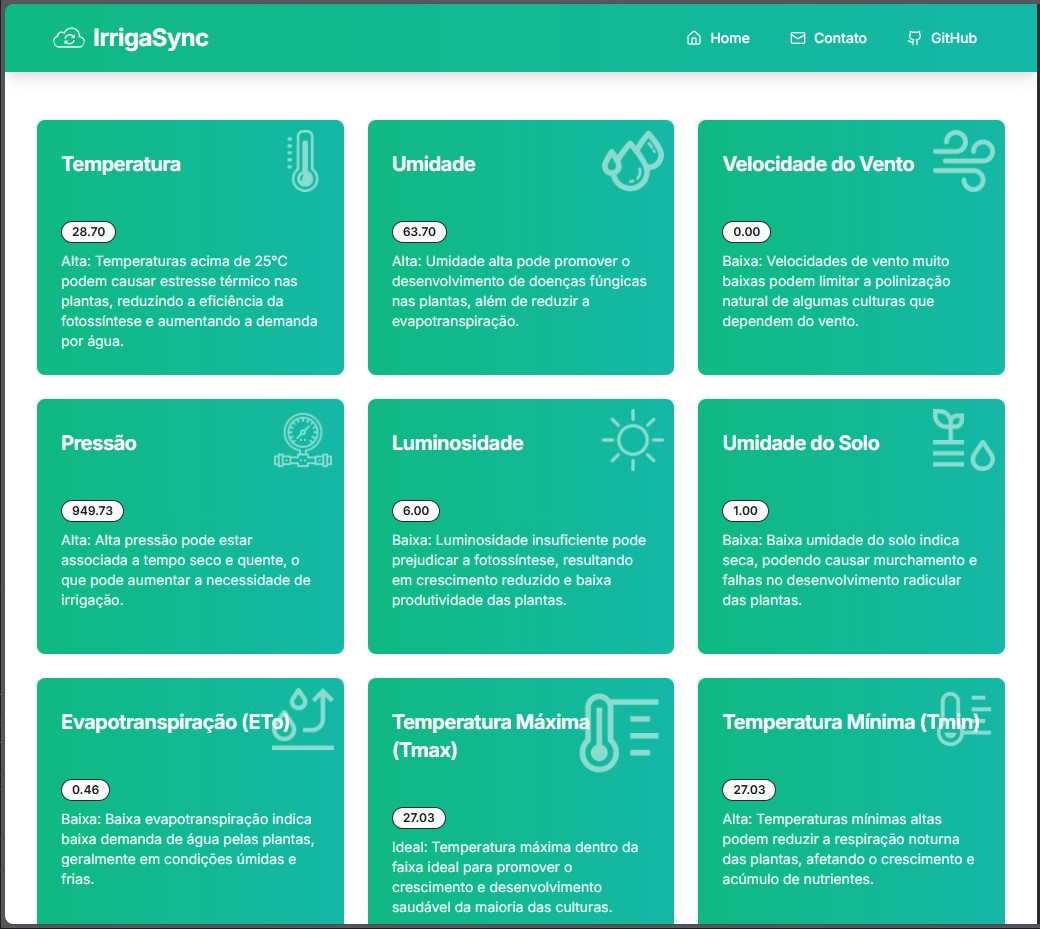
\includegraphics[width=16cm]{figuras/irrigaSync.png}
\fonte{Elaborado pelo autor, 2024.}
\end{varwidth}
\end{figure}

\begin{figure}[!htb] \centering
\caption{\textit{IrrigaSync mobile}} \label{figura:irrigaMobile}
\begin{varwidth}{\linewidth}
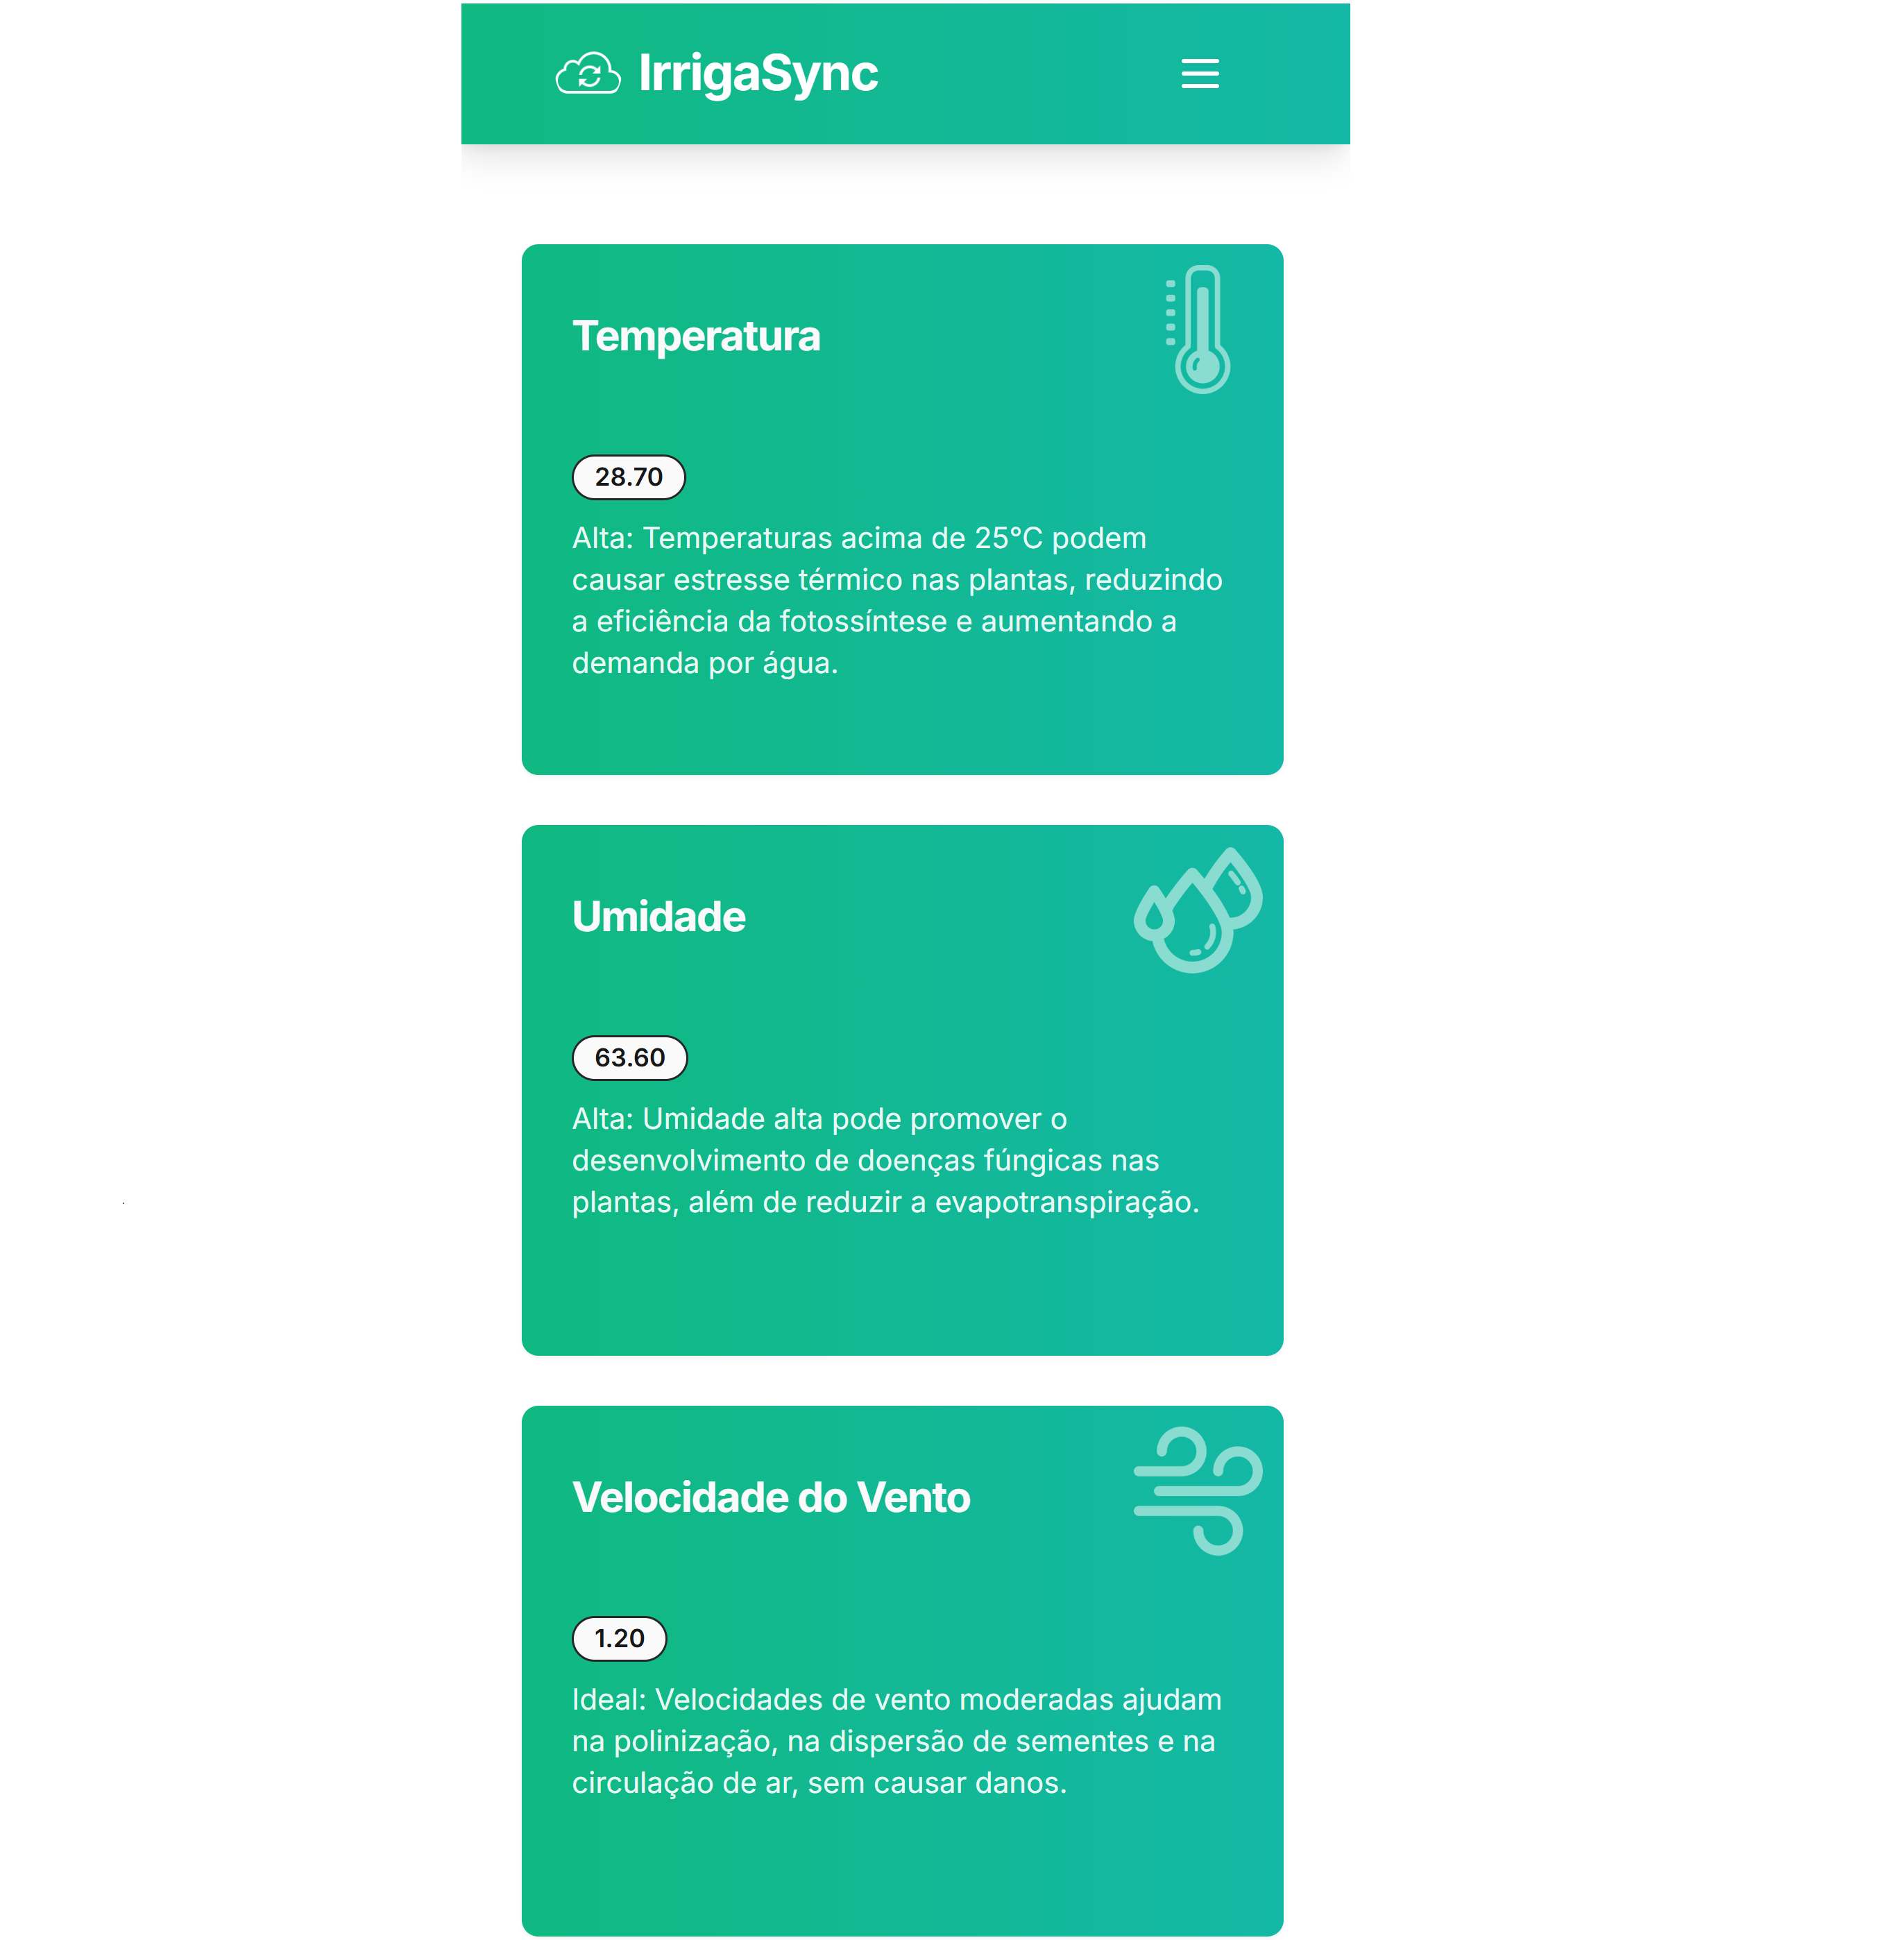
\includegraphics[width=16cm]{figuras/irrigaSyncMobile.png}
\fonte{Elaborado pelo autor, 2024.}
\end{varwidth}
\end{figure}

\section{Montagem do \textit{hardware}}

Para ilustrar o processo de montagem do \textit{hardware}, a Figura \ref{figura:gab-proj} apresenta o gabinete contendo a PCB instalada e os componentes integrados. Essa montagem final foi projetada para oferecer proteção contra intempéries e garantir a estabilidade do sistema.

\begin{figure}[!htb] \centering
\caption{Gabinete com PCB instalado} \label{figura:gab-proj}
\begin{varwidth}{\linewidth}
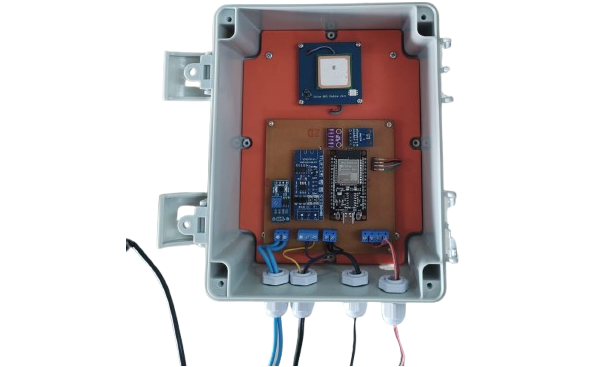
\includegraphics[width=16cm]{figuras/gab-proj.png}
\fonte{Elaborado pelo autor, 2024.}
\end{varwidth}
\end{figure}

\section{Dados coletados}

Os dados meteorológicos capturados diretamente pelo sistema incluem temperatura, umidade relativa do ar, velocidade do vento, luminosidade e pressão atmosférica. A seguir, estão as descrições dos principais resultados obtidos para cada variável durante um dia no local de implementação (16/10/2024).

\subsection{Temperatura e umidade relativa do ar}
Os valores de temperatura e umidade relativa foram obtidos a partir do sensor DHT22. A temperatura variou entre 19\textdegree C e 30\textdegree C, enquanto a umidade relativa oscilou entre 40\% e 85\%. Os gráficos da Figura \ref{fig:leituras-temp} e Figura \ref{fig:leituras-umid} apresenta a evolução desses parâmetros ao longo de um período de 12 horas.

\begin{figure}[!htb] \centering
  \caption{Evolução da temperatura em 12 horas (06:00 - 18:00)} \label{fig:leituras-temp}
  \begin{varwidth}{\linewidth}
    \includegraphics[width=16cm]{figuras/Temperatura_°C.png}
    \fonte{Elaborado pelo autor, 2024.}
  \end{varwidth}
\end{figure}

\begin{figure}[!htb] \centering
  \caption{Evolução da umidade em 12 horas (06:00 - 18:00)} \label{fig:leituras-umid}
  \begin{varwidth}{\linewidth}
    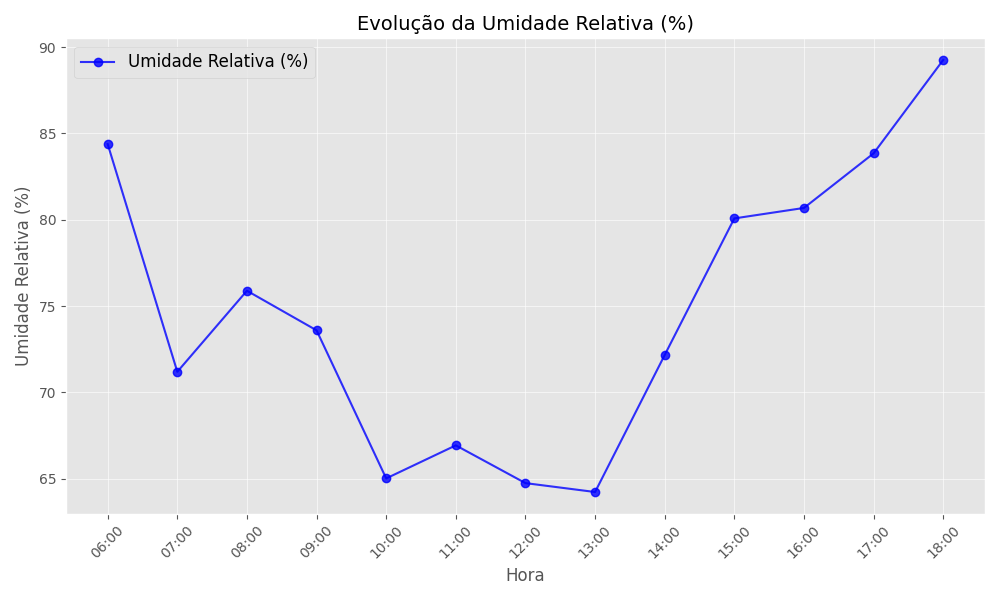
\includegraphics[width=16cm]{figuras/Umidade_Relativa.png}
    \fonte{Elaborado pelo autor, 2024.}
  \end{varwidth}
\end{figure}

\subsection{Velocidade do vento}
As medições de velocidade do vento, capturadas pelo anemômetro RS-FSJT-N01, mostraram uma variação entre 0.5 m/s e 12 m/s. A Figura \ref{fig:leituras-vel} ilustra a distribuição das velocidades ao longo de 12 horas.

\begin{figure}[!htb] \centering
  \caption{Evolução da velocidade do vento em 12 horas (06:00 - 18:00)} \label{fig:leituras-vel}
  \begin{varwidth}{\linewidth}
    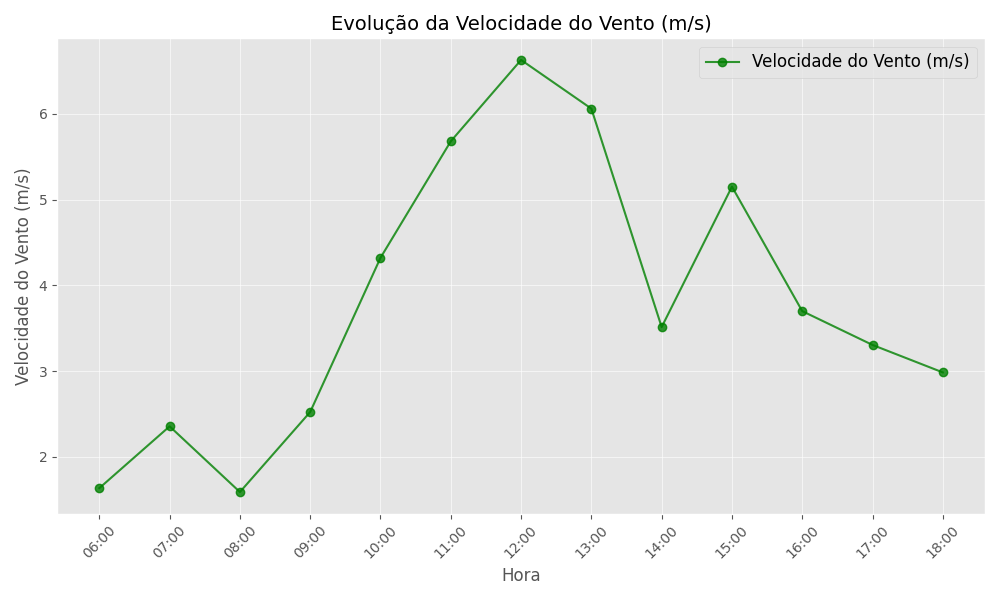
\includegraphics[width=16cm]{figuras/Velocidade_do_Vento_m_s.png}
    \fonte{Elaborado pelo autor, 2024.}
  \end{varwidth}
\end{figure}

\subsection{Luminosidade}
A intensidade luminosa medida pelo sensor BH1750 variou entre 400 lux e 25000 lux, refletindo mudanças na radiação solar ao longo do dia. A Figura \ref{fig:leituras-lum} mostra a evolução da luminosidade em função do tempo.

\begin{figure}[!htb] \centering
  \caption{Evolução da luminosidade em 12 horas (06:00 - 18:00)} \label{fig:leituras-lum}
  \begin{varwidth}{\linewidth}
    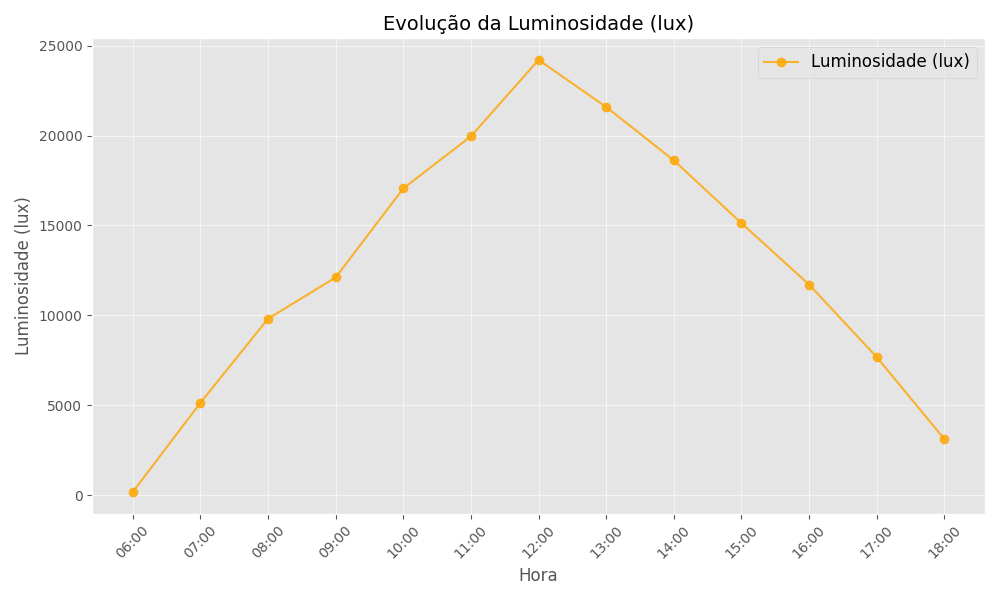
\includegraphics[width=16cm]{figuras/Luminosidade_lux.png}
    \fonte{Elaborado pelo autor, 2024.}
  \end{varwidth}
\end{figure}

\subsection{Pressão atmosférica}
O sensor BMP280 registrou valores de pressão atmosférica entre 950 hPa e 1020 hPa, refletindo as variações da região de Bambuí. A evolução da pressão ao longo do tempo é mostrada na Figura \ref{fig:leituras-pres}.

\begin{figure}[!htb] \centering
    \caption{Evolução das variáveis meteorológicas ao longo de 12 horas (06:00 - 18:00)} \label{fig:leituras-pres}
    \begin{varwidth}{\linewidth}
      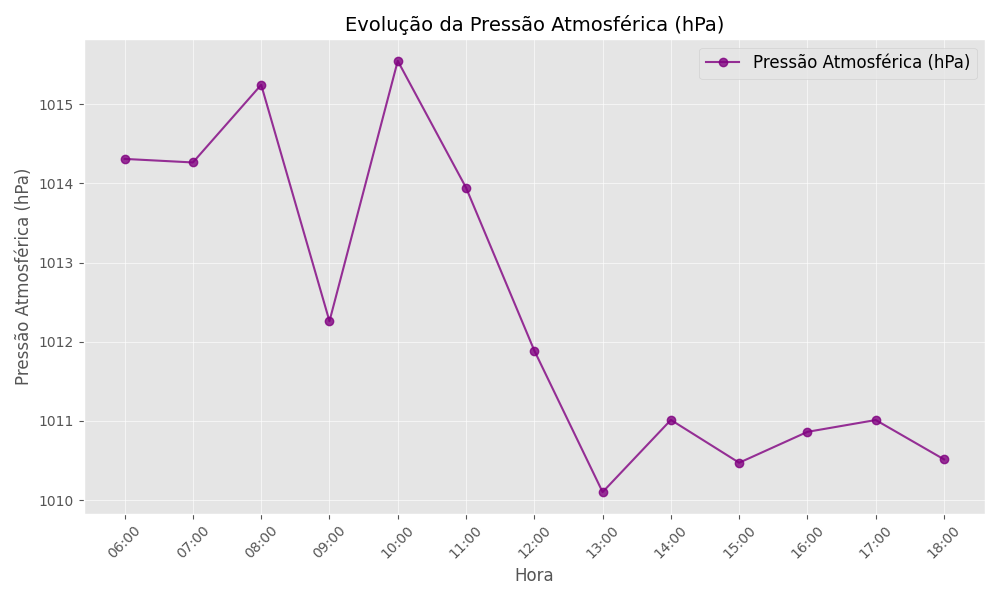
\includegraphics[width=16cm]{figuras/Pressão_Atmosférica_hPa.png}
      \fonte{Elaborado pelo autor, 2024.}
    \end{varwidth}
\end{figure}

\section{Comparação com dados de referência}

Para comparar os dados coletados pelo sistema \textit{IrrigaSync} em 16/10/2024 foram utilizadas informações do \textcite{inmet2024}, cuja estação climática se encontra no IFMG, \textit{Campus} Bambuí. A Tabela \ref{tab:comparacao-dados} apresenta uma comparação entre as variáveis climáticas registradas pelo \textit{IrrigaSync} e os dados disponíveis do INMET para a mesma data e periódo horário.

\begin{table}[!htb] 
  \caption{Comparação dos dados climáticos em Bambuí em 16/10/2024} 
  \label{tab:comparacao-dados} 
  \begin{tabularx}{\textwidth}{|X|X|X|} \hline 
      \textbf{Variável} & \textbf{\textit{IrrigaSync}} & \textbf{INMET} \\ \hline 
      Temperatura Mínima (\textdegree C) & 19 & 20 \\ \hline 
      Temperatura Máxima (\textdegree C) & 33 & 38 \\ \hline 
      Umidade Relativa Mínima (\%) & 65 & 40 \\ \hline 
      Umidade Relativa Máxima (\%) & 85 & 80 \\ \hline 
  \end{tabularx}
  \fonte{Dados do sistema \textit{IrrigaSync} e do \textcite{inmet2024}.}
\end{table}

Observa-se que os dados de temperatura mínima e umidade relativa máxima registrados pelo \textit{IrrigaSync} estão próximos aos valores fornecidos pelo INMET. No entanto, há uma discrepância na temperatura máxima e na umidade relativa mínima. Essa diferença pode ser atribuída a fatores como a localização específica dos sensores do \textit{IrrigaSync}, possíveis microclimas locais ou variações nos horários de medição.

É importante considerar que os dados do INMET são obtidos de estações meteorológicas padronizadas e calibradas regularmente, enquanto o \textit{IrrigaSync} é um sistema em desenvolvimento que pode necessitar de ajustes e calibrações adicionais para melhorar a precisão de suas medições.

\section{Estimativa da evapotranspiração}

Com base nas variáveis coletadas, o sistema calculou a ETo e a ETc para uma pequena plantação de café arábica utilizando o método FAO-56 \parencite{Allen_evapotranspiration1998}. A plantação, situada ao lado do laboratório, corresponde a uma microcultura, cobrindo uma área de aproximadamente 6260,5 m², com condições controladas e específicas (Figura \ref{fig:plantacao-cafe}).

\begin{figure}[!htb] \centering
  \caption{Microcultura de café arábica do IFMG - \textit{Campus} Bambuí} \label{fig:plantacao-cafe}
  \begin{varwidth}{\linewidth}
    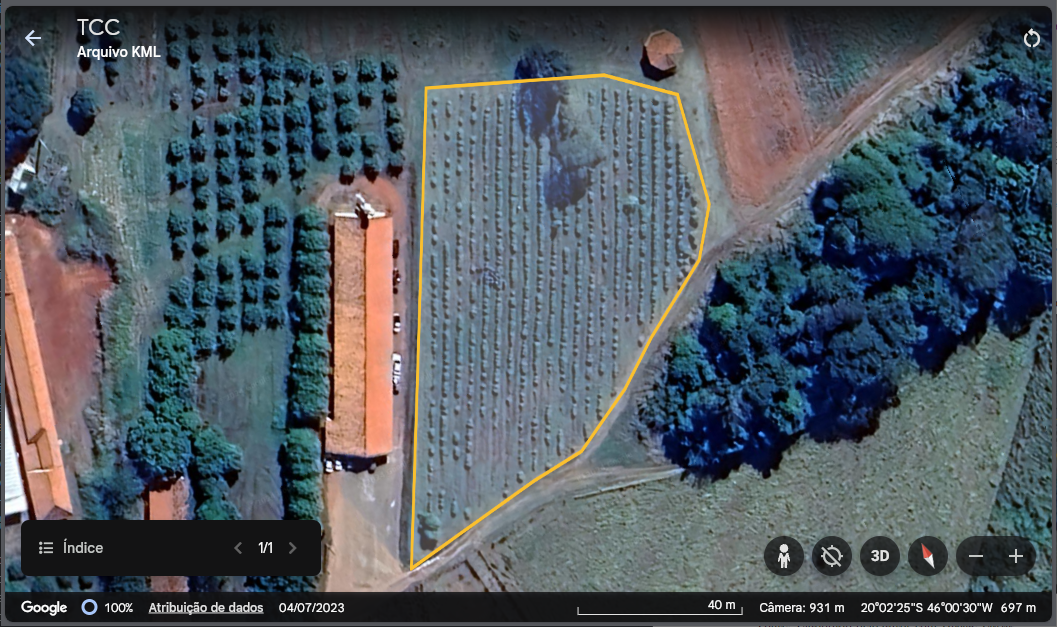
\includegraphics[width=16cm]{figuras/plantacao-cafe.png}
    \fonte{Elaborado pelo autor com \textit{Google Earth}.}
  \end{varwidth}
\end{figure}

De acordo com \textcite{rodrigues2013}, o Kc do café arábica varia de acordo com o estágio de desenvolvimento da planta e o manejo de irrigação. Em lavouras irrigadas, o valor do Kc para o café arábica pode variar ao longo do ano entre 0,21 e 0,80, com uma média de 0,57, dependendo das condições e do manejo da cultura.
No caso específico para essa época do ano, em outubro, geralmente há uma variação dependendo da fase fenológica da planta e das condições climáticas da região. 

Estudos mostram que valores de Kc entre 0,72 e 1,50 são comuns em períodos de maior demanda hídrica, que ocorrem tipicamente entre junho e setembro, mas isso pode se estender, especialmente se houver alta evapotranspiração \parencite{souza2005}. Esses valores podem ser ajustados conforme o manejo de irrigação local, como observado em estudos feitos em Minas Gerais, onde o clima e a metodologia de irrigação impactam bastante o valor do Kc aplicado.

Para adotar um valor médio confiável do Kc para o café arábica utilizando uma abordagem científica, um valor de 0,60 é geralmente uma boa referência durante o ano, especialmente em lavouras irrigadas \parencite{rodrigues2013}. Isso é corroborado por estudos que mostram que o Kc do café arábica varia entre 0,21 e 0,80, com um valor médio ao longo do ciclo produtivo próximo a 0,57. No sistema implementado, o valor de Kc pode ser definido como entrada ao clicar na logo do aplicação na barra de navegação superior, sendo que para a microcultura em questão foi adotado o valor de 0,60.

A Tabela \ref{tab:et} apresenta os valores estimados para ETo e ETc no dia 16/10/2024 para essa microcultura de café arábica capturados pelo sistema \textit{IrrigaSync}.

\begin{table}[!htb]
  \caption{Valores de ETo e ETc coletados pelo sistema \textit{IrrigaSync}} \label{tab:et}
  \begin{tabularx}{\textwidth}{|c|X|X|} \hline
    \textbf{Hora} & \textbf{ETo (mm/dia)} & \textbf{ETc (mm/dia)} \\ \hline
    06:00 & 2.88 & 1.73 \\ \hline
    09:00 & 4.32 & 2.59 \\ \hline
    12:00 & 6.00 & 3.60 \\ \hline
    15:00 & 4.80 & 2.88 \\ \hline
    18:00 & 3.60 & 2.16 \\ \hline
  \end{tabularx}
  \fonte{Resultados obtidos do sistema \textit{IrrigaSync}.}
\end{table}

A escolha do café arábica como cultura monitorada reflete a relevância da sua produção na região. Os dados obtidos podem ser úteis para o manejo preciso de água e o controle climático dessa microcultura, exemplificando a aplicabilidade do sistema \textit{IrrigaSync}.

\section{Discussão dos resultados}

Os resultados apresentados demonstram o funcionamento do sistema \textit{IrrigaSync} para monitoramento ambiental e suporte ao manejo de irrigação em uma microcultura de café arábica. A integração entre o \textit{hardware} e o \textit{software} garantiu a coleta e o processamento de dados relevantes para o contexto agrícola, permitindo a estimativa da evapotranspiração.

A análise dos dados coletados revelou que, embora o sistema atenda aos requisitos funcionais propostos, algumas limitações precisam ser abordadas para garantir maior precisão e confiabilidade. Por exemplo, a comparação com os dados do INMET mostrou discrepâncias em algumas variáveis, como a temperatura máxima e a umidade relativa mínima. Tais diferenças podem ser atribuídas a fatores como localização dos sensores, presença de microclimas locais e calibração inicial dos equipamentos.  

Além disso, a análise da infraestrutura revelou desafios relacionados à cobertura da rede \textit{Wi-Fi} no laboratório, o que limitou a transmissão de dados em tempo real em algumas áreas. 

O sistema também apresentou limitações no sensor de umidade do solo, que registrou variações mais amplas do que o esperado. Isso sugere a necessidade de uma análise mais rigorosa do desempenho desse sensor, incluindo possíveis substituições por modelos mais precisos e adequados ao ambiente em questão.  

Outro ponto relevante é a aplicabilidade do \textit{IrrigaSync} para diferentes culturas agrícolas. Embora o protótipo tenha sido validado em uma microcultura de café arábica, sua modularidade e flexibilidade permitem adaptações para outros tipos de cultivo. No entanto, para garantir a eficácia em diferentes cenários, ajustes nos valores de \textit{Kc} são necessários, considerando fatores específicos de cada cultura.  

